\documentclass[10pt]{beamer}

% Beamer style
%\usetheme[secheader]{Madrid}
% \usetheme{CambridgeUS}
\useoutertheme{infolines}
\usecolortheme[rgb={0.65,0.15,0.25}]{structure}
% \usefonttheme[onlymath]{serif}
\beamertemplatenavigationsymbolsempty
%\AtBeginSubsection

% Packages
%\usepackage[french]{babel}
\usepackage[latin1]{inputenc}
\usepackage{color}
\usepackage{xspace}
%\usepackage{dsfont, stmaryrd}
\usepackage{amsmath, amsfonts, amssymb}
\usepackage{url}
\usepackage{/home/robin/LATEX/Biblio/astats}
%\usepackage[all]{xy}
\usepackage{graphicx}
\usepackage{tikz}
% TikZ
\newcommand{\nodesize}{2em}
\newcommand{\edgeunit}{2*\nodesize}
\tikzstyle{hidden}=[draw, circle, fill=gray!50, minimum width=\nodesize, inner sep=0]
\tikzstyle{observed}=[draw, circle, fill=white,minimum width=\nodesize, inner sep=0]
\tikzstyle{eliminated}=[draw, circle, minimum width=\nodesize, color=gray!50, inner sep=0]
\tikzstyle{empty}=[]
\tikzstyle{arrow}=[->, >=latex, line width=1pt]
\tikzstyle{edge}=[-, line width=1pt]
\tikzstyle{dashededge}=[-, dashed, line width=1pt]
\tikzstyle{dashedarrow}=[->, >=latex, dashed, line width=1pt]
\tikzstyle{lightarrow}=[->, >=latex, line width=1pt, fill=gray!50, color=gray!50]

% % TikZ
% \newcommand{\nodesize}{1.8em}
% \newcommand{\edgeunit}{2.2*\nodesize}
% \tikzstyle{hidden}=[draw, circle, fill=gray!50, minimum width=\nodesize, inner sep=0]
% \tikzstyle{observed}=[draw, circle, minimum width=\nodesize, inner sep=0]
% \tikzstyle{eliminated}=[draw, circle, minimum width=\nodesize, color=gray!50, inner sep=0]
% \tikzstyle{empty}=[]
% \tikzstyle{arrow}=[->, >=latex, line width=1pt]
% \tikzstyle{edge}=[-, line width=1pt]
% \tikzstyle{dashedarrow}=[->, >=latex, dashed, line width=1pt]
% \tikzstyle{lightarrow}=[->, >=latex, line width=1pt, fill=gray!50, color=gray!50]


% \newcommand{\nodesize}{2em}
% \newcommand{\edgeunit}{1*\nodesize}
% \tikzstyle{node}=[point, inner sep=0]
% \tikzstyle{edge}=[-, line width=.5pt]

% Not numbering backup slides
\newcommand{\backupbegin}{
   \newcounter{finalframe}
   \setcounter{finalframe}{\value{framenumber}}
}
\newcommand{\backupend}{
   \setcounter{framenumber}{\value{finalframe}}
}


% Commands
\definecolor{darkred}{rgb}{0.65,0.15,0.25}
\newcommand{\emphase}[1]{\textcolor{darkred}{#1}}
% \newcommand{\emphase}[1]{{#1}}
\newcommand{\paragraph}[1]{\textcolor{darkred}{#1}}
\newcommand{\refer}[1]{{\footnotesize{\textcolor{gray}{[{\cite{#1}}]}}}}
\newcommand{\Refer}[1]{{\footnotesize{\textcolor{gray}{[{#1}]}}}}
\renewcommand{\newblock}{}

% Symbols
\newcommand{\Abf}{{\bf A}}
\newcommand{\Beta}{\text{B}}
\newcommand{\Bcal}{\mathcal{B}}
\newcommand{\BIC}{\text{BIC}}
\newcommand{\Ccal}{\mathcal{C}}
\newcommand{\dd}{\text{~d}}
\newcommand{\dbf}{{\bf d}}
\newcommand{\Dcal}{\mathcal{D}}
\newcommand{\Esp}{\mathbb{E}}
\newcommand{\Espt}{\widetilde{\Esp}}
\newcommand{\Ebf}{{\bf E}}
\newcommand{\Ecal}{\mathcal{E}}
\newcommand{\Gcal}{\mathcal{G}}
\newcommand{\Gam}{\mathcal{G}\text{am}}
\newcommand{\Hcal}{\mathcal{H}}
\newcommand{\Ibb}{\mathbb{I}}
\newcommand{\Ibf}{{\bf I}}
\newcommand{\ICL}{\text{ICL}}
\newcommand{\Cov}{\mathbb{C}\text{ov}}
\newcommand{\Corr}{\mathbb{C}\text{orr}}
\newcommand{\Var}{\mathbb{V}}
\newcommand{\Vsf}{\mathsf{V}}
\newcommand{\pen}{\text{pen}}
\newcommand{\pt}{\widetilde{p}}
\newcommand{\Fcal}{\mathcal{F}}
\newcommand{\Hbf}{{\bf H}}
\newcommand{\Jcal}{\mathcal{J}}
\newcommand{\Kbf}{{\bf K}}
\newcommand{\Lcal}{\mathcal{L}}
\newcommand{\Mcal}{\mathcal{M}}
\newcommand{\mbf}{{\bf m}}
\newcommand{\mum}{\mu(\mbf)}
\newcommand{\Ncal}{\mathcal{N}}
\newcommand{\Nbf}{{\bf N}}
\newcommand{\Nm}{N(\mbf)}
\newcommand{\Ocal}{\mathcal{O}}
\newcommand{\Obf}{{\bf 0}}
\newcommand{\Omegas}{\underset{s}{\Omega}}
\newcommand{\Pbf}{{\bf P}}
\newcommand{\Pt}{\widetilde{P}}
\newcommand{\Pcal}{\mathcal{P}}
\newcommand{\Qcal}{\mathcal{Q}}
\newcommand{\Rbb}{\mathbb{R}}
\newcommand{\Rcal}{\mathcal{R}}
\newcommand{\Scal}{\mathcal{S}}
\newcommand{\Tcal}{\mathcal{T}}
\newcommand{\Ucal}{\mathcal{U}}
\newcommand{\Vcal}{\mathcal{V}}
\newcommand{\BP}{\text{BP}}
\newcommand{\EM}{\text{EM}}
\newcommand{\VEM}{\text{VEM}}
\newcommand{\VBEM}{\text{VBEM}}
\newcommand{\cst}{\text{cst}}
\newcommand{\obs}{\text{obs}}
\newcommand{\ra}{\emphase{\mathversion{bold}{$\rightarrow$}~}}
%\newcommand{\transp}{\text{{\tiny $\top$}}}
\newcommand{\transp}{\text{{\tiny \mathversion{bold}{$\top$}}}}
\newcommand{\logit}{\text{logit}\xspace}

% Directory
\newcommand{\figmixt}{/home/robin/ENSEIGN/COURS/MELANGE}
\newcommand{\figbma}{/home/robin/RECHERCHE/RUPTURES/MELANGE/Exemples/Grippe}
\newcommand{\fignet}{../FIGURES}
\newcommand{\figeco}{/home/robin/RECHERCHE/ECOLOGIE/EXPOSES/FIGURES}
%\newcommand{\figmotif}{/home/robin/RECHERCHE/RESEAUX/Motifs/FIGURES}


%====================================================================
%====================================================================

%====================================================================
%====================================================================
\begin{document}
%====================================================================
%====================================================================

%====================================================================
\title[Statistical network inference]{Statistical network inference}

\author[SR]{UMR MIA-Paris: S. Ouadah, S. Robin, ...}

\institute[INRA/AgroParisTech]{INRA / AgroParisTech \\ ~\\
  \vspace{-.1\textwidth}
  \begin{tabular}{ccccc}
%     
\includegraphics[height=.3\textheight]{\fignet/LogoINRA-Couleur} & 
%     \hspace{.02\textheight} &
%     
\includegraphics[height=.08\textheight]{\fignet/logagroptechsolo} & 
%     \hspace{.02\textheight} &
%     
\includegraphics[height=.09\textheight]{\fignet/logo-ssb}
    
\includegraphics[height=.2\textheight]{\fignet/LogoINRA-Couleur} & 
    \hspace{.02\textheight} &
    
\includegraphics[height=.067\textheight]{\fignet/logagroptechsolo} & 
    \hspace{.02\textheight} &
    
\includegraphics[height=.06\textheight]{\fignet/logo-ssb}
    \\ 
  \end{tabular} \\
  \bigskip
  }

\date[AgroParisTech, Nov.'16]{Learn Biocontrol, AgroParisTech, November 2016}

%====================================================================
%====================================================================
\maketitle
%====================================================================
\frame{\frametitle{Outline} \tableofcontents}

%====================================================================
%====================================================================
\section{Statistics for networks}
\frame{\frametitle{Outline} \tableofcontents[currentsection]}
%====================================================================
\frame{ %\frametitle{Different questions}

  \paragraph{Network:} convenient way to describe 
  $$
  \text{connexions / relations / interactions \quad \ra \quad links } i \sim j
  $$
  between 
  $$
  \text{individuals / genes / species / entities \quad \ra \quad nodes } i
  $$
  
  \bigskip \bigskip \pause
  \paragraph{'Network' = graph $G$:} 
  $$
  G = (V, E)
  $$
  $V = \{1, \dots p\} =$ set of nodes, $E =$ set of edges.

  \bigskip \bigskip  \pause
  \paragraph{Alternatively:} Adjacency matrix
  $$
  A = [A_{ij}]:
  \qquad
  A_{ij} = \left\{
    \begin{array}{cl} 
     1 & \text{if } i \sim j,\\
     0 & \text{otherwise.}\\
    \end{array}
  \right.
  $$
  
}
  
%====================================================================
\frame{ \frametitle{Different questions}

  \paragraph{Understanding the network topology:}
  \begin{itemize}
   \item Data = observed network
   \item Questions: central nodes? cluster structure? small-world property? ...
  \end{itemize}

  \bigskip \pause
  \paragraph{Inferring the network:}
  \begin{itemize}
   \item Data = repeated signal observed at each node
   \item Questions: which nodes are connected?
  \end{itemize}

  \bigskip \pause
  \paragraph{Using the network:}
  \begin{itemize}
   \item Data = a given network + signal on nodes
   \item Questions: how the epidemic spreads along the network?
  \end{itemize}
  
  \bigskip \pause
  \paragraph{Each to be combined with}
  covariates, time, missing data, ...

}

%====================================================================
\section{Network inference}
\frame{\frametitle{Outline} \tableofcontents[currentsection]}
%====================================================================
\frame{ \frametitle{A brief review}

  \paragraph{Data.} $p$ species ($i = 1 .. p$), $n$ replicates ($r = 1..n$)
  \begin{eqnarray*}
   Y_{ir} & = & \text{abundance of species $i$ in replicate $r$} \\
   Y_r = (Y_{ir})_{i=1..p} & = & \text{vector of abundances in replicate $r$}
  \end{eqnarray*}
  
  \bigskip
  \paragraph{Goal.} Infer the \emphase{species interaction network} from the set of $Y_r$?   \refer{VTK16}
  
  \bigskip \bigskip
  \paragraph{Remarks.}
  \begin{itemize}
   \item Need to specify the type of interaction
   \item Need to distinguish between direct and indirect interactions
  \end{itemize}
}
  
%====================================================================
\frame{ \frametitle{General framework: Graphical models \refer{Lau96}}

  \paragraph{Example:} (undirected graph) \\
  \vspace{-.1\textheight}
  \begin{tabular}{cc}
    \begin{tabular}{p{.5\textwidth}}
    \hspace{-.1\textwidth}
    \includegraphics[width=.6\textwidth]{../FIGURES/FigGGM-4nodes}
    \end{tabular}
    & 
    \hspace{-.05\textwidth}
    \begin{tabular}{p{.4\textwidth}}
    \pause
    \paragraph{Properties:} ~ 
    
    \bigskip
    All variables are dependent (connected graph).
    
    \bigskip \pause
    Some are conditionally independent, e.g.
    $$
    Y_4 \perp (Y_1, Y_2) | Y_3
    $$
    \end{tabular}
  \end{tabular} 

}
  
%====================================================================
\frame{ \frametitle{Graphical models}

  \bigskip
  \paragraph{More precisely.} $P =$ joint distribution faithful to $G$ iff
  $$
  P(Y_1, \dots, Y_p) \propto \prod_{C \in \Ccal_G} \psi_C(Y_C)
  $$
  where $\Ccal_G =$ set of cliques of $G$. \refer{HaC71}
  
  \bigskip \bigskip \pause
  \paragraph{Example.} ~ \\
  \vspace{-.2\textheight}
  \begin{tabular}{cc}
    \begin{tabular}{p{.5\textwidth}}
    \hspace{-.1\textwidth}
    \includegraphics[width=.6\textwidth]{../FIGURES/FigGGM-4nodes}
    \end{tabular}
    & 
    \hspace{-.05\textwidth}
    \begin{tabular}{p{.4\textwidth}}
    $P(Y_1, Y_2, Y_3, Y_4) \propto$
    $$
    \psi_1(Y_1 ,Y_2, Y_3) \times \psi_2(Y_3, Y_4)
    $$
    \end{tabular}
  \end{tabular} 
  
}

%====================================================================
\frame{ \frametitle{Network inference}

  \paragraph{Data.} $Y_{ir} = $ (say) abundance of species $i$ in replicate $r$.
%   \begin{itemize}
%    \item $Y_{ir} = $ (say) abundance of species $i$ in replicate $r$
%    \item $Y_r = (Y_{1r}, \dots Y_{pr}) =$ vector of abundance in replicate $r$
%   \end{itemize}

  \bigskip \bigskip \pause
  \paragraph{Generic statistical model.}
  $$
  (Y_r)_{r = 1..n} \text{ iid } \sim P, 
  \qquad
   P \text{ is faithful to } G
   $$

  \bigskip \bigskip \pause
  \paragraph{Network inference problem.}
  $$
  \text{Based on the dataset $Y = (Y_{ir})$, infer $G$.}
  $$

  \bigskip \bigskip \pause
  \paragraph{Critical issue.} There are $2^{p(p-1)/2}$ possible graphs
  $$
  \begin{array}{lcccc}
    p & 5 & 10 & 20 & 50 \\ \hline
    \text{\# graphs} & 10^3 & 10^{14} & 10^{57} & 10^{369}
  \end{array}
  $$
}

%====================================================================
\section{Gaussian graphical models}
\frame{\frametitle{Outline} \tableofcontents[currentsection]}
%====================================================================
\frame{ \frametitle{GGM = Gaussian graphical models}

  \paragraph{Gaussian distribution.}
  $$
  Y_r \sim \Ncal_p(\mu, \Sigma)
  $$
  $\mu =$ vector of means, $\Sigma =$ covariance matrix.
  
  \bigskip \bigskip \pause
  \paragraph{A nice property.} ~ \\
  \vspace{-.2\textheight}
  \begin{tabular}{cc}
    \begin{tabular}{p{.5\textwidth}}
    \hspace{-.15\textwidth}
    \includegraphics[width=.6\textwidth]{../FIGURES/FigGGM-4nodes}
    \end{tabular}
    & 
    \hspace{-.15\textwidth}
    \begin{overprint}
    \onslide<2>
    \begin{tabular}{p{.5\textwidth}}
	 Adjacency matrix
	 $$
	 A = \left[ \begin{array}{cccc}
	 0 & 1 & 1 & \emphase{0} \\
	 1 & 0 & 1 & \emphase{0} \\
	 1 & 1 & 0 & 1 \\
	 \emphase{0} & \emphase{0} & 1 & 0 
	 \end{array} \right]
	 $$
    \end{tabular} 
    \onslide<3>
    \begin{tabular}{p{.5\textwidth}}
	 Covariance matrix
	 $$
	 \Sigma \propto \left[ \begin{array}{cccc}
	   1 & -.25 & -.41 &  \emphase{.25} \\
	   -.25 &  1 & -.41 &  \emphase{.25} \\
	   -.41 & -.41 &  1 & -.61 \\
	   \emphase{.25} &  \emphase{.25} & -.61 &  1
	   \end{array} \right] 
	 $$
    \end{tabular} 
    \onslide<4>
    \begin{tabular}{p{.5\textwidth}}
	 Inverse covariance matrix
	 $$
	 \Sigma^{-1} \propto \left[ \begin{array}{cccc}
	   1 & .5 & .5 & \emphase{0} \\
	   .5 & 1 & .5 & \emphase{0} \\
	   .5 & .5 & 1 & .5 \\
	   \emphase{0} & \emphase{0} & .5 & 1
	   \end{array} \right] 
	 $$
    \end{tabular} 
    \onslide<5>
    \begin{tabular}{p{.5\textwidth}}
	 Estimated inverse covariance matrix
	 $$
	 \widehat{\Sigma}^{-1} \propto \left[ \begin{array}{cccc}
	   1 & .48 & .61 & \emphase{.09} \\
	   .48 & 1 & .67 & \emphase{.06} \\
	   .61 & .67 & 1 & .46 \\
	   \emphase{.09} & \emphase{.06} & .46 & 1
	   \end{array} \right] 
	 $$
	 ($n = 100$)
    \end{tabular} 
    \end{overprint}
  \end{tabular}

% $$
% \widehat{\Sigma} \propto \left[ \begin{array}{cccc}
%   1 & -.02 & -.49 & .25 \\
%   -.02 & 1 & -.62 & .36 \\
%   -.49 & -.62 & 1 & -.61 \\
%   .25 & .36 & -.61 & 1
%   \end{array} \right] 
% $$
}

%====================================================================
\frame{ \frametitle{Sparsity}

  \paragraph{Sparsity assumption:}
  $$
  \Omega = \Sigma^{-1} \text{ is sparse}
  $$
  = most entries of $\Omega$ are zeros.
  
  \bigskip \bigskip \pause
  \paragraph{A series of approaches} for Gaussian data
  \begin{itemize}
   \item Sparse regression of each species on the others:
   $$
   Y_i = a_j + \sum_{j \neq i} b_{ij} Y_j + E_i \quad \text{forcing most $b_{ij} = 0$ \refer{MeB06}}
   $$
   \item Directly estimate $\Omega$ forcing most $\omega_{ij} = 0$ \refer{FHT08}
  \end{itemize}
  using, e.g, Lasso penalty \refer{Tib96,EHJ04} or more refined \refer{ACM09}.

}

%====================================================================
\section{Tree-based Bayesian inference}
\frame{\frametitle{Outline} \tableofcontents[currentsection]}
%====================================================================
\frame{ \frametitle{Inference of tree-shaped network \refer{MeJ06,SRS15}}

  \paragraph{Same problem.} Infer $G$ based on an iid sample $(Y_r) \sim P$ faithful to $G$.

  \bigskip \bigskip \pause
  \paragraph{Tree assumption:} The network $G$ is a spanning tree, i.e.
  $$
  \left. \begin{tabular}{l}
          $G$ is connected \\
          $G$ has no cycle
         \end{tabular} \right\}
  \text{\ra $G$ has $p-1$ edges (sparse)}
  $$

  \bigskip \bigskip \pause
  \paragraph{Bayesian inference:} aim at providing
  \begin{itemize}
   \item the global posterior distribution of $G$ given the data $Y$: $P(G|Y)$
   \item or edge probabilities:
   $$
   P(i \sim j | Y)
   $$
  \end{itemize}
}

%====================================================================
\frame{ \frametitle{Tree-shaped network}

  \begin{tabular}{c||c}
    Spanning trees & Non spanning trees \\ & \\ \hline
    \hspace{-.05\textwidth}
    \begin{tabular}{l|l}
    \includegraphics[width=.23\textwidth]{../FIGURES/FigGGM-Chain.pdf} &
    \hspace{-.05\textwidth}
    \includegraphics[width=.23\textwidth]{../FIGURES/FigGGM-Star.pdf} \\ \hline
    \includegraphics[width=.23\textwidth]{../FIGURES/FigGGM-Tree.pdf} & 
    \includegraphics[width=.23\textwidth]{../FIGURES/FigGGM-LargerTree.pdf}
    \end{tabular}
    & 
    \hspace{-.05\textwidth}
    \begin{tabular}{l|l}
    \includegraphics[width=.23\textwidth]{../FIGURES/FigGGM-TreeNonSpanning.pdf} & 
    \hspace{-.05\textwidth}
    \includegraphics[width=.23\textwidth]{../FIGURES/FigGGM-NonTree.pdf} \\ \hline
    \includegraphics[width=.23\textwidth]{../FIGURES/FigGGM-Loop.pdf} & 
    \includegraphics[width=.23\textwidth]{../FIGURES/FigGGM-FullGraph.pdf}
    \end{tabular}
  \end{tabular}


}

%====================================================================
\frame{ \frametitle{Exact Bayesian inference}

  \paragraph{Bayesian inference} requires to sum over all possible graphs \\
  \ra sum over all possible spanning trees ($\# \Tcal = p^{p-2}$).
  
  \bigskip \bigskip \pause
  \paragraph{An algebraic tool.} $w_{ij} =$ weight of $(i, j)$
  \begin{itemize}
   \item Score of a tree = product of the weights of its branches
   $$
   s(T) = \prod_{(i, j) \in T} w_{ij}
   $$
   \item Matrix-tree theorem:
   $$
   \sum_{T \in \Tcal} s(T) \text{ is computable in $O(p^3)$}
   $$
  \end{itemize}
}

%====================================================================
\frame{\frametitle{Illustration: Raf pathway \refer{SRS15}}

Flow cytometry data for $p = 11$ proteins from the Raf signaling pathway \refer{SPP05} \\ ~

\begin{tabular}{cc}
  \includegraphics[trim = 12mm 35mm 12mm 18mm, clip,width=0.45\linewidth]{\fignet/RAF.pdf}
  & 
  \includegraphics[width=0.45\linewidth]{\fignet/RAF_edge_prob_graph_q0_05.pdf} \\
  'ground truth' & posterior probabilities \\ 
  ~\\
  \includegraphics[width=0.45\linewidth]{\fignet/best_1.pdf} 
  &
  \includegraphics[width=0.45\linewidth]{\fignet/best_2.pdf} \\
  most likely tree & second most likely tree
\end{tabular}

}

%====================================================================
\section{Extensions}
\frame{\frametitle{Outline} \tableofcontents[currentsection]}
%====================================================================
% \frame{ \frametitle{Omitting nodes}

%   \begin{overprint}
%    \onslide<1>
%     \paragraph{All nodes observed.} ~\\
%     \begin{tabular}{cc}
%     \hspace{-.1\textwidth}
%     \begin{tabular}{p{.5\textwidth}}
% 	 \includegraphics[width=.5\textwidth]{../FIGURES/FigGGM-Complete.pdf}
%     \end{tabular}
%     & 
%     \hspace{-.1\textwidth} 
%     \begin{tabular}{p{.5\textwidth}}
%     Gaussian case: \\ 
%     {\footnotesize
%     	 $$
% 	 \Sigma \propto \left[ \begin{array}{rrrrrrr}
% 	 1 & .4 & .4 & -.2 & -.2 & -.6 & .4 \\ 
% 	 & 1 & .4 & -.2 & -.2 & -.6 & .4 \\ 
% 	 & & 1 & -.2 & -.2 & -.6 & .4 \\ 
% 	 & & & 1 & .3 & .4 & -.5 \\ 
% 	 & & & & 1 & .4 & -.5 \\ 
% 	 & & & & & 1 & -.7 \\ 
% 	 & & & & & & 1
% 	   \end{array} \right] 
% 	 $$
%     	 $$
% 	 \Omega \propto \left[ \begin{array}{rrrrrrr}
% 	 1 & \emphase{0} & \emphase{0} & \emphase{0} & \emphase{0} & .4 & \emphase{0} \\ 
% 	 & 1 & \emphase{0} & \emphase{0} & \emphase{0} & .4 & \emphase{0} \\ 
% 	 & & 1 & \emphase{0} & \emphase{0} & .4 & \emphase{0} \\ 
% 	 & & & 1 & \emphase{0} & \emphase{0} & .4 \\ 
% 	 & & & & 1 & \emphase{0} & .4 \\ 
% 	 & & & & & 1 & .4 \\ 
% 	 & & & & & & 1 
% 	 \end{array} \right] 
% 	 $$
% 	 }
%     \end{tabular}
%     \end{tabular}
% %%%%%%%%%%%%%%%%%%%%%%%%%%%%%%%%%%%%%%%%%%%%%%%
%      \onslide<2>
%     \paragraph{Node 7 missing.} ~\\
%     \begin{tabular}{cc}
%     \hspace{-.1\textwidth}
%     \begin{tabular}{p{.5\textwidth}}
% 	 \includegraphics[width=.5\textwidth]{../FIGURES/FigGGM-1missing.pdf}
%     \end{tabular}
%     & 
%     \hspace{-.1\textwidth} 
%     \begin{tabular}{p{.5\textwidth}}
%     Gaussian case: \\ 
%     {\footnotesize
%     	 $$
% 	 \Sigma \propto \left[ \begin{array}{rrrrrr}
% 	 1 & .4 & .4 & -.2 & -.2 & -.6 \\ 
% 	 & 1 & .4 & -.2 & -.2 & -.6 \\ 
% 	 & & 1 & -.2 & -.2 & -.6 \\ 
% 	 & & & 1 & .3 & .4 \\ 
% 	 & & & & 1 & .4 \\ 
% 	 & & & & & 1
% 	 \end{array} \right] 
% 	 $$
%     	 $$
% 	 \Omega \propto \left[ \begin{array}{rrrrrr}
% 	 1 & \emphase{0} & \emphase{0} & \emphase{0} & \emphase{0} & .4 \\ 
% 	 & 1 & \emphase{0} & \emphase{0} & \emphase{0} & .4 \\ 
% 	 & & 1 & \emphase{0} & \emphase{0} & .4 \\ 
% 	 & & & 1 & -.2 & -.2 \\ 
% 	 & & & & 1 & -.2 \\ 
% 	 & & & & & 1
% 	 \end{array} \right] 
% 	 $$
% 	 }
%     \end{tabular}
%     \end{tabular}
% %%%%%%%%%%%%%%%%%%%%%%%%%%%%%%%%%%%%%%%%%%%%%%%%%%%%%%%
%    \onslide<3>
%     \paragraph{Nodes 6 \& 7 missing.} ~\\
%     \begin{tabular}{cc}
%     \hspace{-.1\textwidth}
%     \begin{tabular}{p{.5\textwidth}}
% 	 \includegraphics[width=.5\textwidth]{../FIGURES/FigGGM-2missing.pdf}
%     \end{tabular}
%     & 
%     \hspace{-.1\textwidth} 
%     \begin{tabular}{p{.5\textwidth}}
%     Gaussian case: \\ 
%     {\footnotesize
%     	 $$
% 	 \Sigma \propto \left[ \begin{array}{rrrrr}
% 	 1 & .4 & .4 & -.2 & -.2 \\ 
% 	 & 1 & .4 & -.2 & -.2 \\ 
% 	 & & 1 & -.2 & -.2 \\ 
% 	 & & & 1 & .3 \\ 
% 	 & & & & 1	   
% 	 \end{array} \right] 
% 	 $$
%     	 $$
% 	 \Omega \propto \left[ \begin{array}{rrrrr}
% 	 1 & -.2 & -.2 & .1 & .1 \\ 
% 	 & 1 & -.2 & .1 & .1 \\ 
% 	 & & & .1 & .1 \\ 
% 	 & & & 1 & -.2 \\ 
% 	 & & & & 1 
% 	 \end{array} \right] 
% 	 $$
% 	 }
%     \end{tabular}
%     \end{tabular}
%   \end{overprint}
% }
  
%====================================================================
\frame{ \frametitle{Removing nodes}

  \begin{overprint}
   \onslide<1>
    \paragraph{Complete network (all nodes).} ~\\ ~\\
    \begin{tabular}{cc}
    \begin{tabular}{p{.5\textwidth}}
	 Graphical model \\
	 \includegraphics[width=.4\textwidth]{../FIGURES/FigGraphModel-5nodes.pdf}
    \end{tabular}
    & 
    \begin{tabular}{p{.5\textwidth}}
    \end{tabular}
    \end{tabular}
   \onslide<2>
    \paragraph{Removing one node.} ~\\ ~\\
    \begin{tabular}{cc}
    \begin{tabular}{p{.5\textwidth}}
	 Marginal graph (missing node) \\
	 \includegraphics[width=.4\textwidth]{../FIGURES/FigGraphModel-5nodesMarg4.pdf}
    \end{tabular}
    & 
    \hspace{-.1\textwidth}
    \begin{tabular}{p{.5\textwidth}}
	 Conditional graph (observed node) \\
	 \includegraphics[width=.4\textwidth]{../FIGURES/FigGraphModel-5nodesCond4.pdf}
    \end{tabular}
    \end{tabular}
   \onslide<3>
    \paragraph{Removing one node.} ~\\ ~\\
    \begin{tabular}{cc}
    \begin{tabular}{p{.5\textwidth}}
	 Marginal graph (missing node) \\
	 \includegraphics[width=.4\textwidth]{../FIGURES/FigGraphModel-5nodesMarg5.pdf}
    \end{tabular}
    & 
    \hspace{-.1\textwidth}
    \begin{tabular}{p{.5\textwidth}}
	 Conditional graph (observed node) \\
	 \includegraphics[width=.4\textwidth]{../FIGURES/FigGraphModel-5nodesCond5.pdf}
    \end{tabular}
    \end{tabular}
   \onslide<4->
    \paragraph{Removing one node.} ~\\ ~\\
    \begin{tabular}{cc}
    \begin{tabular}{p{.5\textwidth}}
	 Marginal graph (missing node) \\
	 \includegraphics[width=.4\textwidth]{../FIGURES/FigGraphModel-5nodesMarg3.pdf}
    \end{tabular}
    & 
    \hspace{-.1\textwidth}
    \begin{tabular}{p{.5\textwidth}}
	 Conditional graph (observed node) \\
	 \includegraphics[width=.4\textwidth]{../FIGURES/FigGraphModel-5nodesCond3.pdf}
    \end{tabular}
    \end{tabular}
  \end{overprint}

  \bigskip   
  \onslide+<5>
  More complex patterns for directed graphical models.

}
  
%====================================================================
\frame{ \frametitle{Accounting for covariates (1/3)}

  \paragraph{Deciphering the pathobiome:} Intra-and interkingdom interactions involving the pathogen {\sl E. alphitoides}. \refer{JFS16}
  
  \bigskip \bigskip \pause
  \paragraph{Data.}
  \begin{itemize}
   \item 3 trees $\times$ few tens of leaves per tree
   \item Abundance of few tens of (fungal and bacterial) species on each leaves via NGS
   \item Few covariates describing both trees and leaves
  \end{itemize}

  \bigskip \bigskip \pause
  \paragraph{Questions.}
  \begin{itemize}
   \item Infer the ecological network
   \item Account for covariates (to avoid spurious edges)
   \item Deal with NGS counts as $(Y_{ir})$ measurements
  \end{itemize}
}
  
%====================================================================
\frame{ \frametitle{Accounting for covariates (2/3)}

  \paragraph{Proposed strategy.}
  \begin{enumerate}
   \item Perform regression on the covariates $x$ for each species $i$:
   $$
   Y_{ir} \sim \Pcal(\mu_{ir}), \qquad \log \mu_{ir} = x_r \beta_i
   \qquad \rightarrow \qquad
   \widehat{\mu}_{ir} = e^{x_r \widehat{\beta}_i}
   $$
   \item Compute the Pearson residuals $\widetilde{Y}_{ir} = (Y_{ir} - \widehat{\mu}_{ir}) / \sqrt{\widehat{\mu}_{ir}}$
   \item Infer the network from the corrected abundances $(\widetilde{Y}_{ir})$ using \refer{SRS15}.
  \end{enumerate}

  \bigskip \bigskip \pause
  \paragraph{Still unsolved problem.}
  \begin{itemize}
   \item How to account for the uncertainty of the $\widehat{\beta}_i$ in the inference of $G$?
  \end{itemize}
}

%====================================================================
\frame{ \frametitle{Accounting for covariates (3/3)}

    \begin{tabular}{cc}
    \hspace{-.05\textwidth}
    \begin{tabular}{p{.6\textwidth}}
      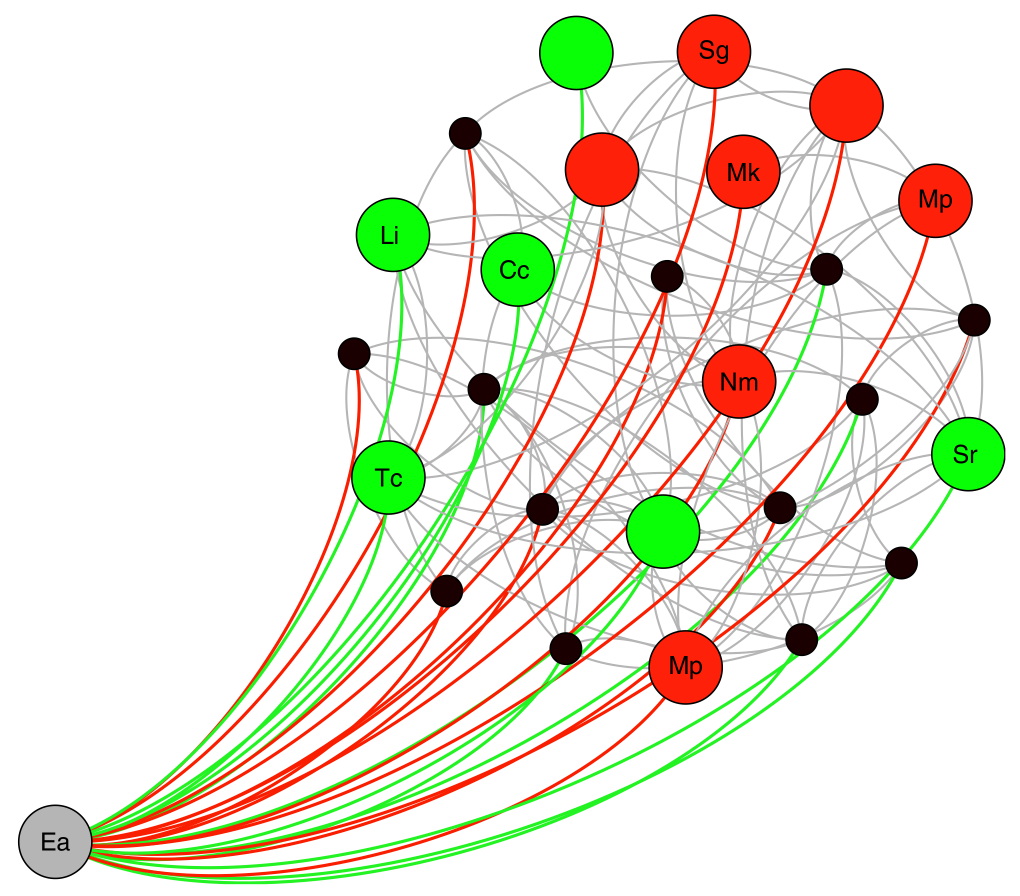
\includegraphics[width=.5\textwidth]{../FIGURES/JFS16-EnvirMicrobiol-Fig4.pdf}
    \end{tabular}
    & 
    \hspace{-.05\textwidth}
    \begin{tabular}{p{.35\textwidth}}
    \textcolor{gray}{{\Huge $\bullet$}}: {\sl E. alphitoides} \\ ~
    
    \textcolor{red}{{\Huge $\bullet$}}: positively correlated fungal OTUs \\ ~
    
    \textcolor{green}{{\Huge $\bullet$}}: negatively correlated fungal OTUs \\ ~
    
    {{\Large $\bullet$}}: bacterial OTUs
    \end{tabular}
  \end{tabular}

}

%====================================================================
\frame{ \frametitle{Missing nodes (1/3)}

  \begin{tabular}{cc}
    \begin{tabular}{p{.45\textwidth}}
    \paragraph{Fact.} Block-structured empirical correlation matrix. \\~
    
    \ra Each block could be associated with an unobserved node. \\ ~ 

    \ra Can we infer such missing nodes? \\ ~ 

    \end{tabular}
    & 
    \hspace{-.05\textwidth}
    \begin{tabular}{p{.5\textwidth}}
	 \includegraphics[width=.5\textwidth]{../FIGURES/FigGGM-ObservedCor-2missing.pdf}
    \end{tabular}
  \end{tabular}
}
  
%====================================================================
\frame{ \frametitle{Missing nodes (2/3)}

  \paragraph{Problem statement.} 
  There exist a complete vector 
  $$
  (\underset{O = \text{observed}}{\underbrace{Y_1, \dots Y_p}}, \underset{H = \text{hidden}}{\underbrace{Z_1, \dots Z_r}})
  $$ 
  the distribution $P$ of which is faithful to a graph $G$.

  \bigskip \bigskip \pause
  \paragraph{EM algorithm.} \refer{Rob16}
  \begin{itemize}
   \item E-step: infer $H$ from $O$ with current parameters ($\mu, \Sigma, G, ...$)
   \item M-step: update the parameters using $O$ and $\widehat{H}$ (using \refer{SRS15} for $G$).
  \end{itemize}

}
  
%====================================================================
\frame{ \frametitle{Missing nodes (3/3)}

  \begin{tabular}{cc}
    \hspace{-.05\textwidth}
    \begin{tabular}{p{.5\textwidth}}
	 \includegraphics[width=.4\textwidth]{../FIGURES/raf_net.jpg}
    \end{tabular}
    & 
    \hspace{-.2\textwidth}
    \begin{tabular}{p{.5\textwidth}}
	 \includegraphics[width=.4\textwidth]{../FIGURES/raf_marg.jpg}
    \end{tabular}
    \\
    \begin{tabular}{p{.4\textwidth}}
	 Accuracy for edge detection based on edge probability:
    \end{tabular}
    & 
    \hspace{-.05\textwidth} 
    \begin{tabular}{p{.6\textwidth}}
	 \vspace{-.1\textheight}
	 \includegraphics[width=.4\textwidth, height=.4\textheight]{../FIGURES/cyto_HC_marginal_graph.jpg}
    \end{tabular}
  \end{tabular}

}

%====================================================================
\frame{ \frametitle{Change-point detection (1/2)}

  \paragraph{Data:} $Y_t = (Y_{1t}, \dots Y_{pt})$ collected along time $t$.
  
  \bigskip \pause
  \paragraph{Problem:} Suppose that $Y_t$ is associated with graph $G_t$, that is affected by abrupt changes:
  $$
  \includegraphics[width=.9\textwidth]{../FIGURES/ScR16-Fig1.pdf}
  $$
  \ra Infer both the change-points and the network associated with each period \refer{RLR11,ScR16}

}
  
%====================================================================
\frame{\frametitle{Change-point detection (2/2)} 

  \paragraph{Data:} $N = 67$ time points, $p = 11$ genes, four expected regions

  \pause \bigskip
  Posterior probability of change-points:
  $$
  \includegraphics[width=.7\textwidth]{../FIGURES/ScR16-Fig9.pdf}
  $$
  \pause
  Inferred networks:
  $$
  \includegraphics[width=.8\textwidth]{../FIGURES/ScR16-Fig8.pdf}
  $$
}

%====================================================================
\section{Concluding remarks \& questions}
%====================================================================
\frame{ \frametitle{Concluding remarks \& questions}
 
  \paragraph{A generic framework} for network inference, with not completely solved problems:
  \begin{itemize}
   \item Deal with NGS counts (non Gaussian)
   \item Accounting for covariates
   \item Incompletely observed species and/or variables
  \end{itemize}

  \bigskip \bigskip \pause
  \paragraph{Questions \& remarks.}
  \begin{itemize}
   \item Network = set of \emphase{binary} interactions
   \item What is an ecological network?
  \end{itemize}
}
  
%====================================================================
%====================================================================
\frame[allowframebreaks]{ \frametitle{References}
{\tiny
  \bibliography{/home/robin/Biblio/BibGene}
%   \bibliographystyle{/home/robin/LATEX/Biblio/astats}
  \bibliographystyle{plain}
  }
}


%====================================================================
%====================================================================
\end{document}
%====================================================================
%====================================================================

  \begin{tabular}{cc}
    \begin{tabular}{p{.5\textwidth}}
    \end{tabular}
    & 
    \hspace{-.05\textwidth}
    \begin{tabular}{p{.5\textwidth}}
    \end{tabular}
  \end{tabular}
